\newpage
\section{The Other Side---Solving Equations}\label{A:otherSide}


In this activity, we will explore ideas related to solving equations.


\begin{prob}
Solve the following equation three ways: Using algebra, using the
balance, and with the graph. At each step, the three models should be in
complete alignment.
\[
\]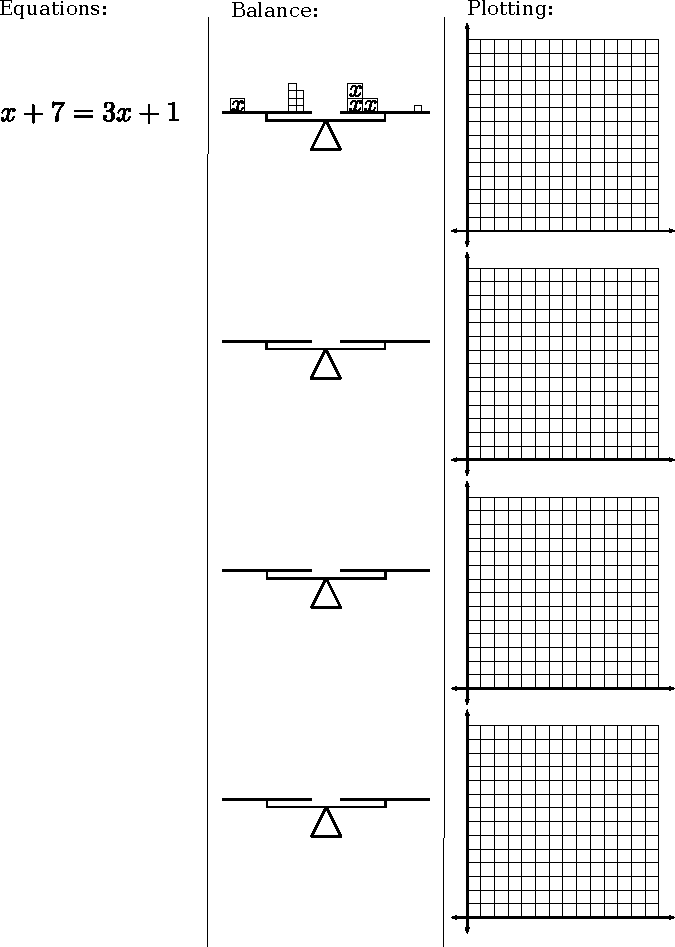
\includegraphics[scale=0.8]{../graphics/eqBalGraph.pdf}
\end{prob}


\begin{prob}
Critically analyze the three ``different'' methods of solving
equations, noting the advantages and disadvantages of each. 
\end{prob}

\begin{prob}
Can you solve quadratic equations using the methods above?
If so give an example. If not, explain why not.
\end{prob}

\begin{teachingnote}
The key point here is that it is difficult to make ``balances'' work for anything but linear equations.  But the graphical approach always works, as described in the following standard:  

CCSS.A-REI.11.  Explain why the $x$-coordinates of the points where the graphs of the equations $y = f(x)$ and $y = g(x)$ intersect are the solutions of the equation $f(x) = g(x)$; find the solutions approximately, e.g., using technology to graph the functions, make tables of values, or find successive approximations. Include cases where $f(x)$ and/or $g(x)$ are linear, polynomial, rational, absolute value, exponential, and logarithmic functions.*
\end{teachingnote}


\begin{prob}
Can you think of an example when the undoing via algebraic
manipulation would fail?
\end{prob}

\begin{teachingnote}
Here we are looking for something where an inverse function must be
applied, as in $.6 = \sin(x)$.
\end{teachingnote}


While sometimes we solve equations via a process of algebraic
manipulation, other times we have a formula.


\begin{prob}
Give a formula for solving linear equations of the form $ax + b =0$.
\end{prob}




